\chapter{Procedure}

\section{RLC Circuit Analysis}

\subsection{Transfer Function Derivation}
In order to derive the voltage gain transfer function ($H_{V}(s)$), we must first convert the circuit from time domain to the s-domain. The circuit is shown in Figure \ref{fig:rlc_circuit}.

\begin{figure}[h]
    \centering
    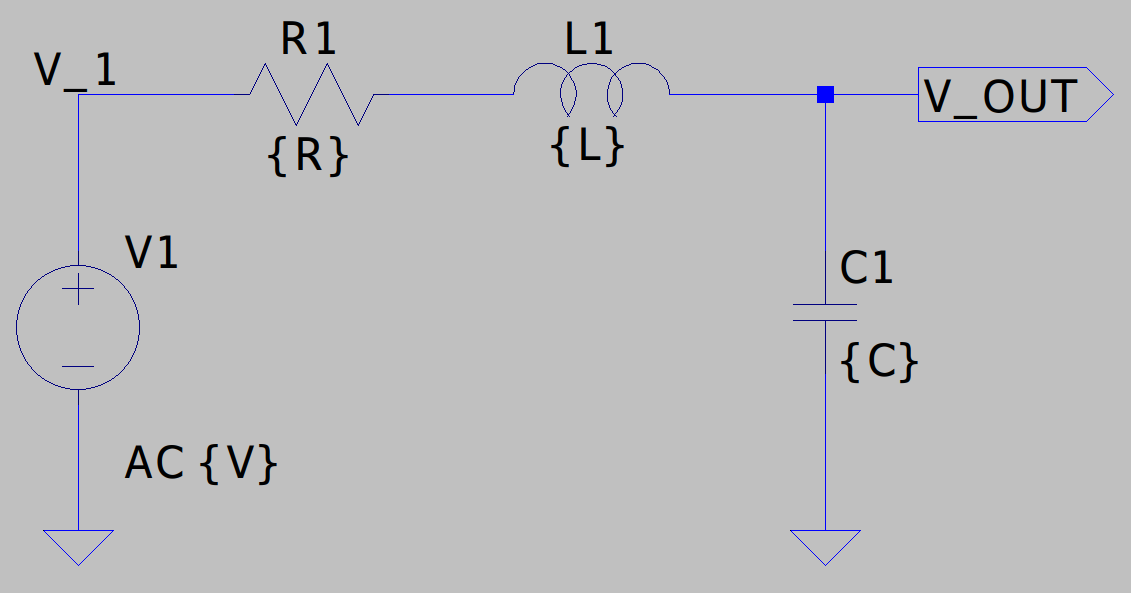
\includegraphics[width=1\textwidth]{assets/rlc-circ.png}
    \caption{RLC Circuit}
    \label{fig:rlc_circuit}
\end{figure}

\noindent Where:
\begin{itemize}
    \item $V_{1}$ is $1 V_{pp}$ input voltage.
    \item $V_{out}$ is the output voltage.
    \item $R$ is $1k\Omega$ resistor.
    \item $L$ is $1mH$ inductor.
    \item $C$ is $0.1\mu F$ capacitor.
\end{itemize}

\newpage
\thispagestyle{plain}

To find the transfer function, we first transform the circuit to the s-domain. The impedance of the resistor, inductor, and capacitor are given by:
\begin{align*}
    Z_{R} &= R \\
    Z_{L} &= sL \\
    Z_{C} &= \frac{1}{sC}
\end{align*}

And the KVL equation for the circuit is:
\begin{align*}
    V_{1} &= V_{R} + V_{L} + V_{C} \\
    V_{1} &= IZ_{R} + IZ_{L} + IZ_{C} \\
    V_{1} &= I(R + sL + \frac{1}{sC}) \\
\end{align*}

Where $I$ is the current through the circuit. The voltage gain transfer function is then:
\begin{align*}
    H_{V}(s) = \frac{V_{out}}{V_{1}} &= \frac{I\frac{1}{sC}}{I(R + sL + \frac{1}{sC})} \\
    &= \frac{\frac{1}{sC}}{R + sL + \frac{1}{sC}} \\
    &\boxed{H_{V}(s) = \frac{1}{sRC + s^{2}LC + 1}}
\end{align*}

\subsection{AC Sweep Analysis Simulation}
To validate the transfer function, we will perform an AC Sweep analysis in LTSpice. The AC Sweep analysis will sweep the frequency of the input voltage from $101Hz$ to $120kHz$. The output voltage will be measured and compared to the transfer function.

\begin{figure}[h]
    \centering
    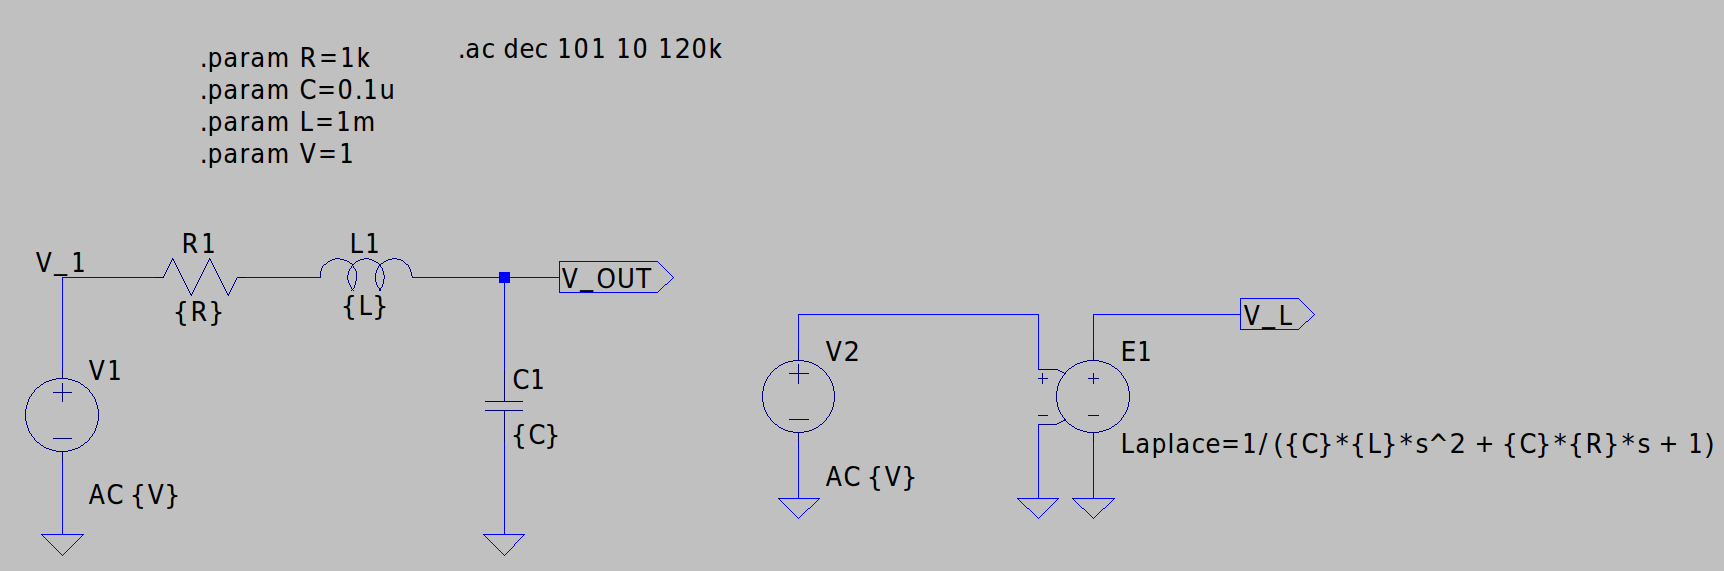
\includegraphics[width=1\textwidth, height=0.3\textheight]{assets/rlc-sim.png}
    \caption{AC Sweep Analysis Simulation Setup}
    \label{fig:ac_sweep}
\end{figure}


\newpage
\thispagestyle{plain}

\begin{figure}[h]
    \centering
    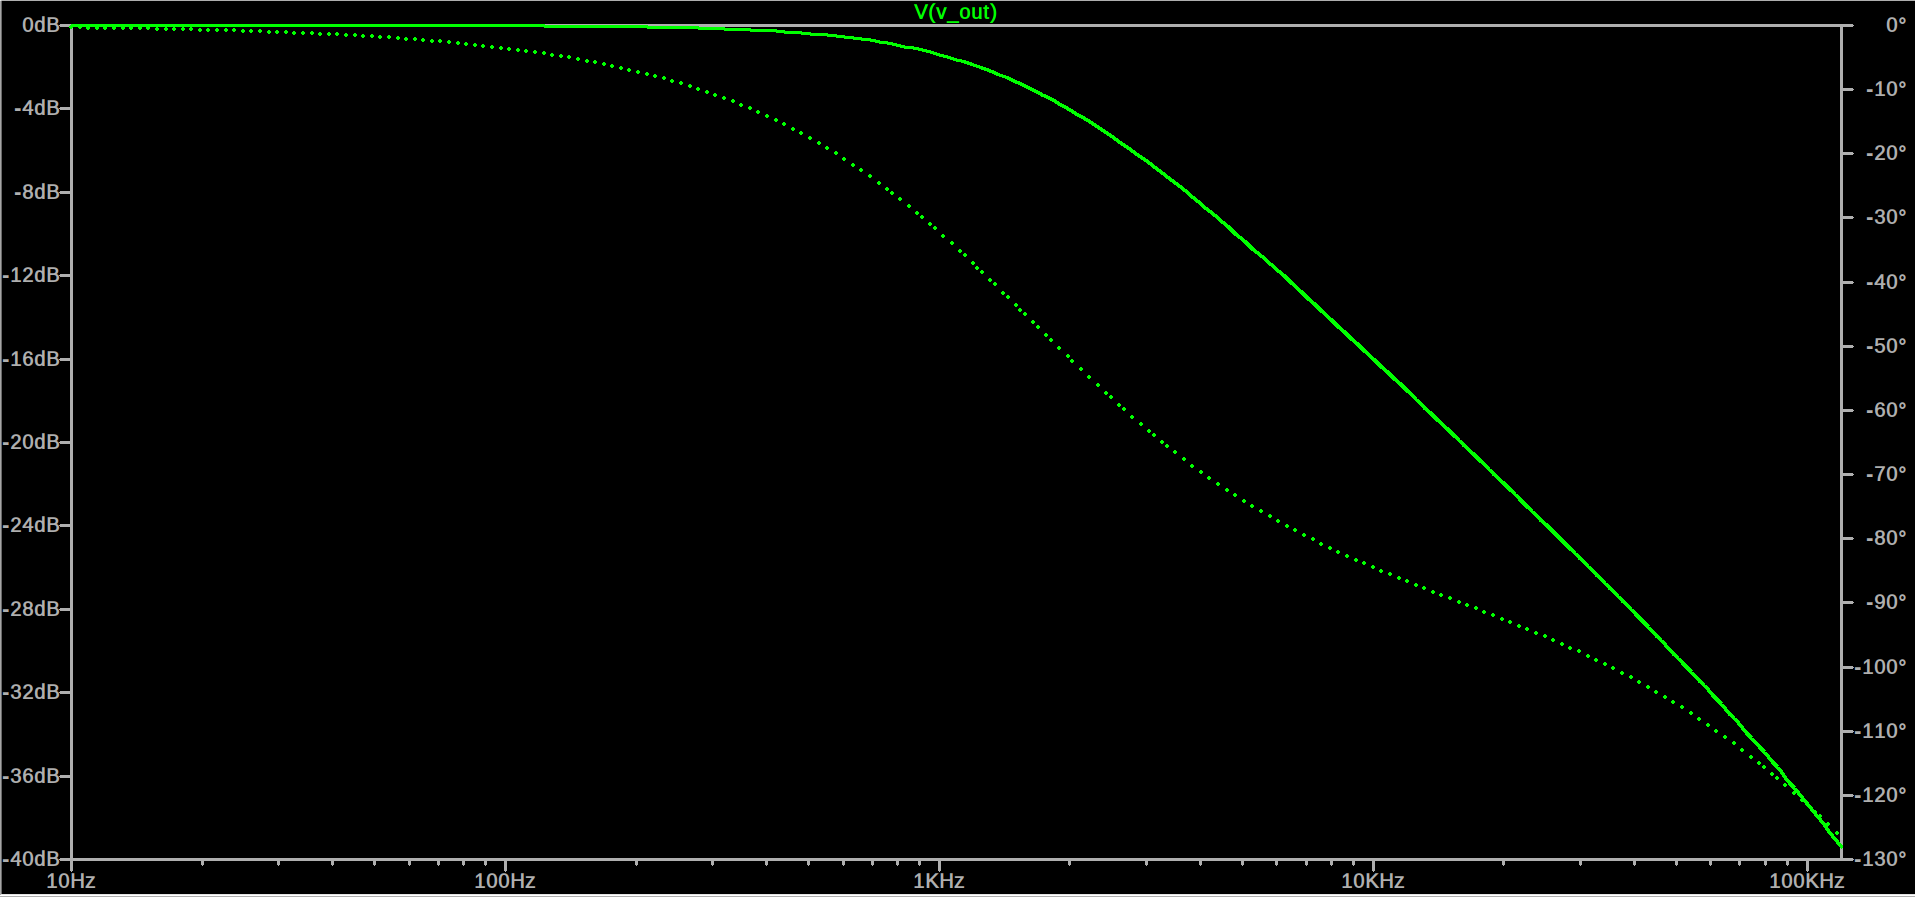
\includegraphics[width=1\textwidth]{assets/rlc-v-out.png}
    \caption{$V_{out}$ Bode Plot}
    \label{fig:rlc_v_out_bode_plot}
\end{figure}
\begin{figure}[h]
    \centering
    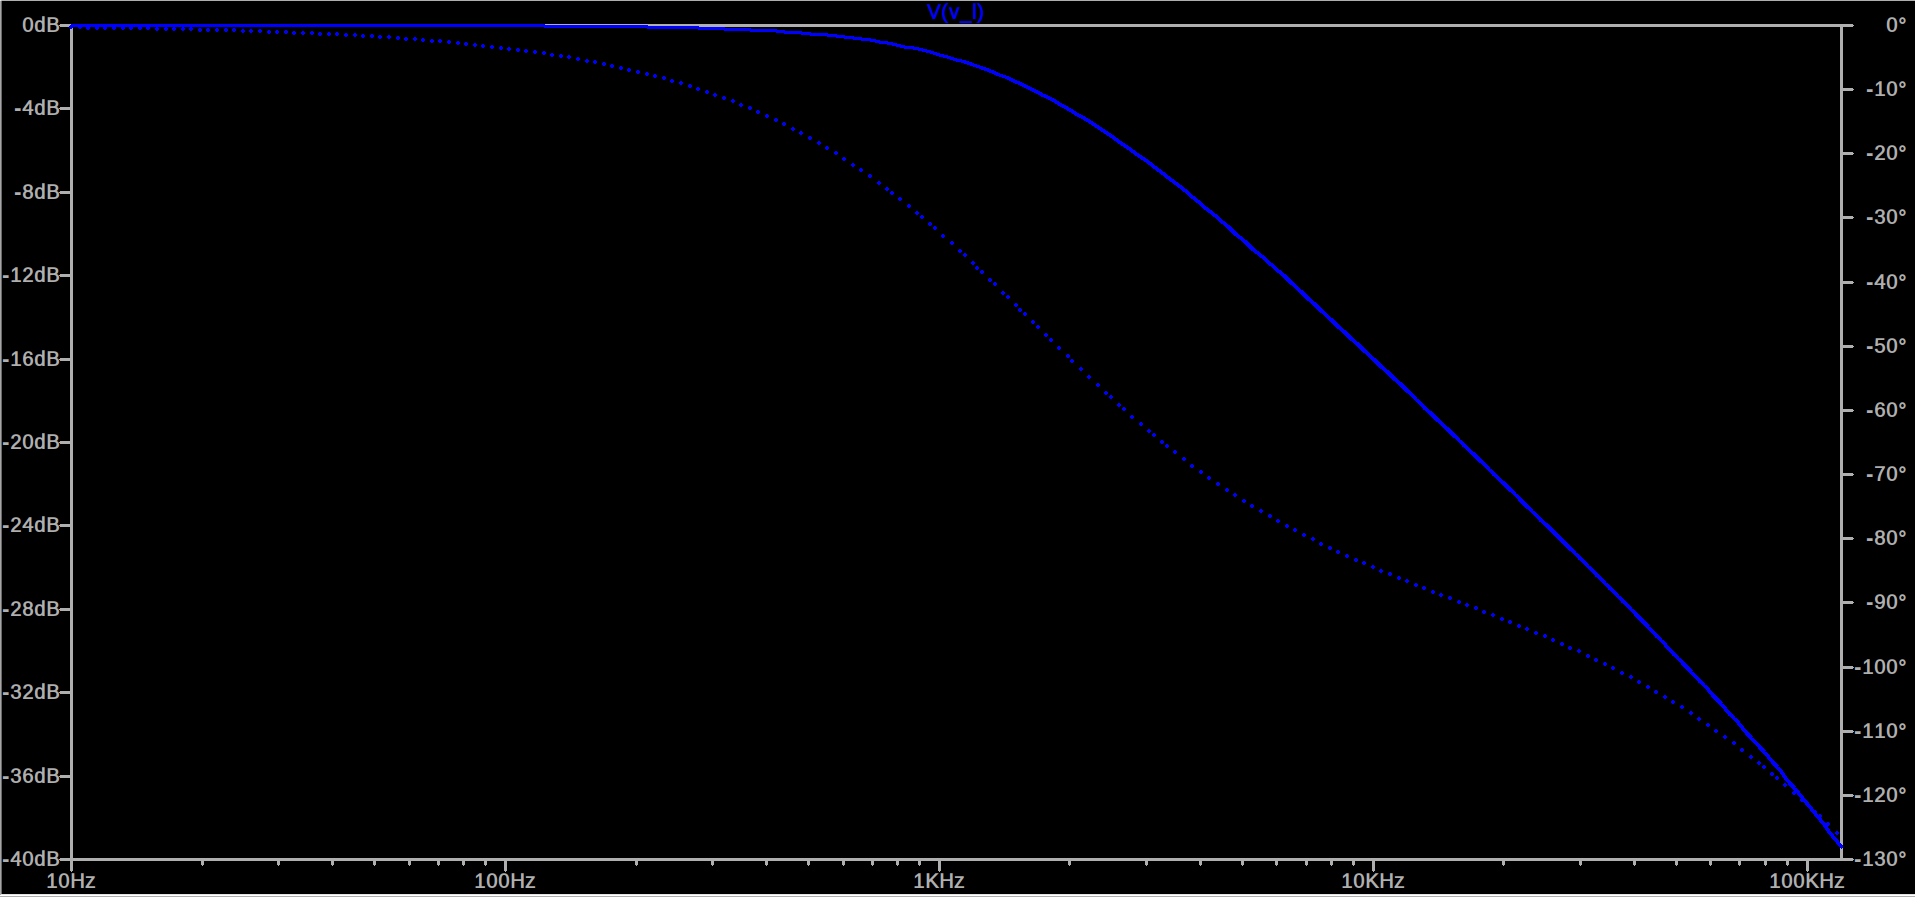
\includegraphics[width=1\textwidth]{assets/rlc-v-l.png}
    \caption{$H_{V}(s)$ Bode Plot}
    \label{fig:rlc_v_laplace_bode_plot}
\end{figure}

As shown in Figure \ref{fig:rlc_v_out_bode_plot}, output voltage frequency response matches the transfer function $H_{V}(s)$ as shown in Figure \ref{fig:rlc_v_laplace_bode_plot}.

\newpage
\thispagestyle{plain}

\subsection{Transient Analysis Simulation}
To further validate the transfer function, we will perform a transient analysis in LTSpice. Changed the input voltage $V_{ac}$ to a $1V_{pp}$ sine wave at $10kHz$. The output voltage will be measured and compared to the transfer function.

\begin{figure}[h]
    \centering
    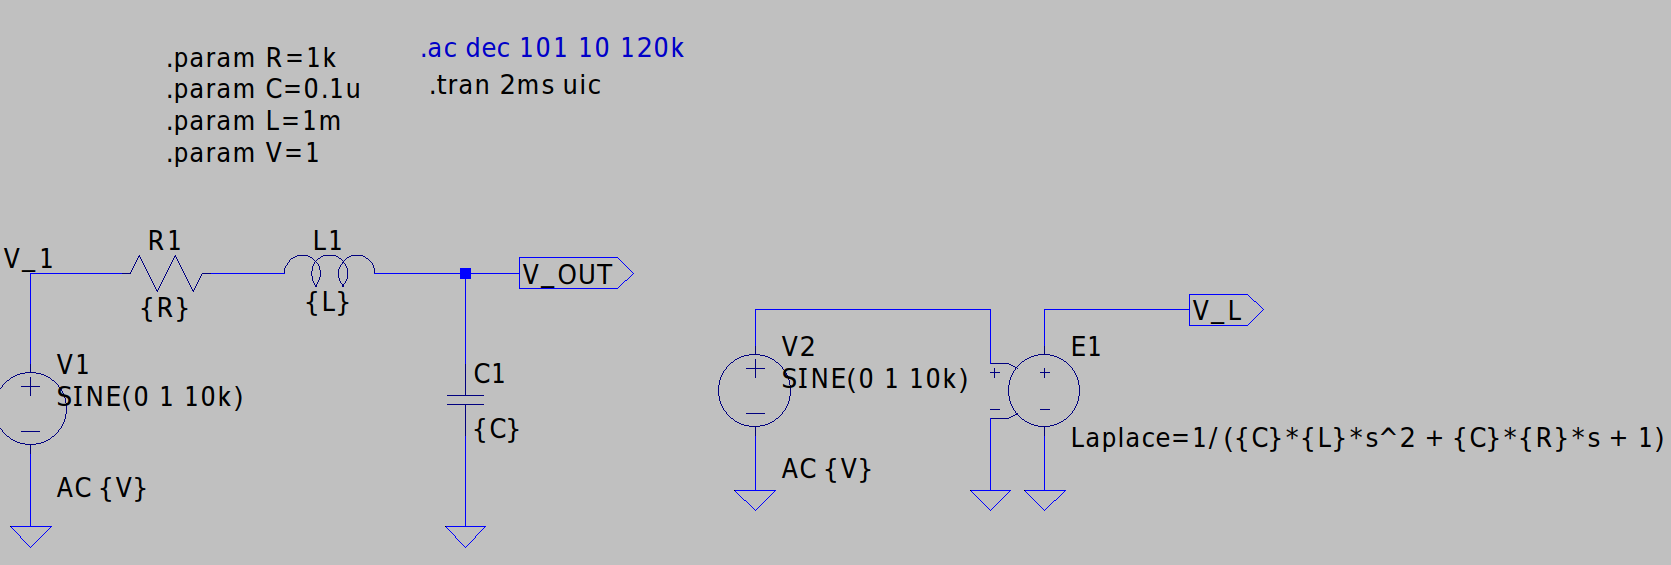
\includegraphics[width=1\textwidth, height=0.4\textheight]{assets/rlc-transient-sim.png}
    \caption{Transient Analysis Simulation Setup}
    \label{fig:transient_analysis}
\end{figure}

\newpage
\thispagestyle{plain}

\begin{figure}[h]
    \centering
    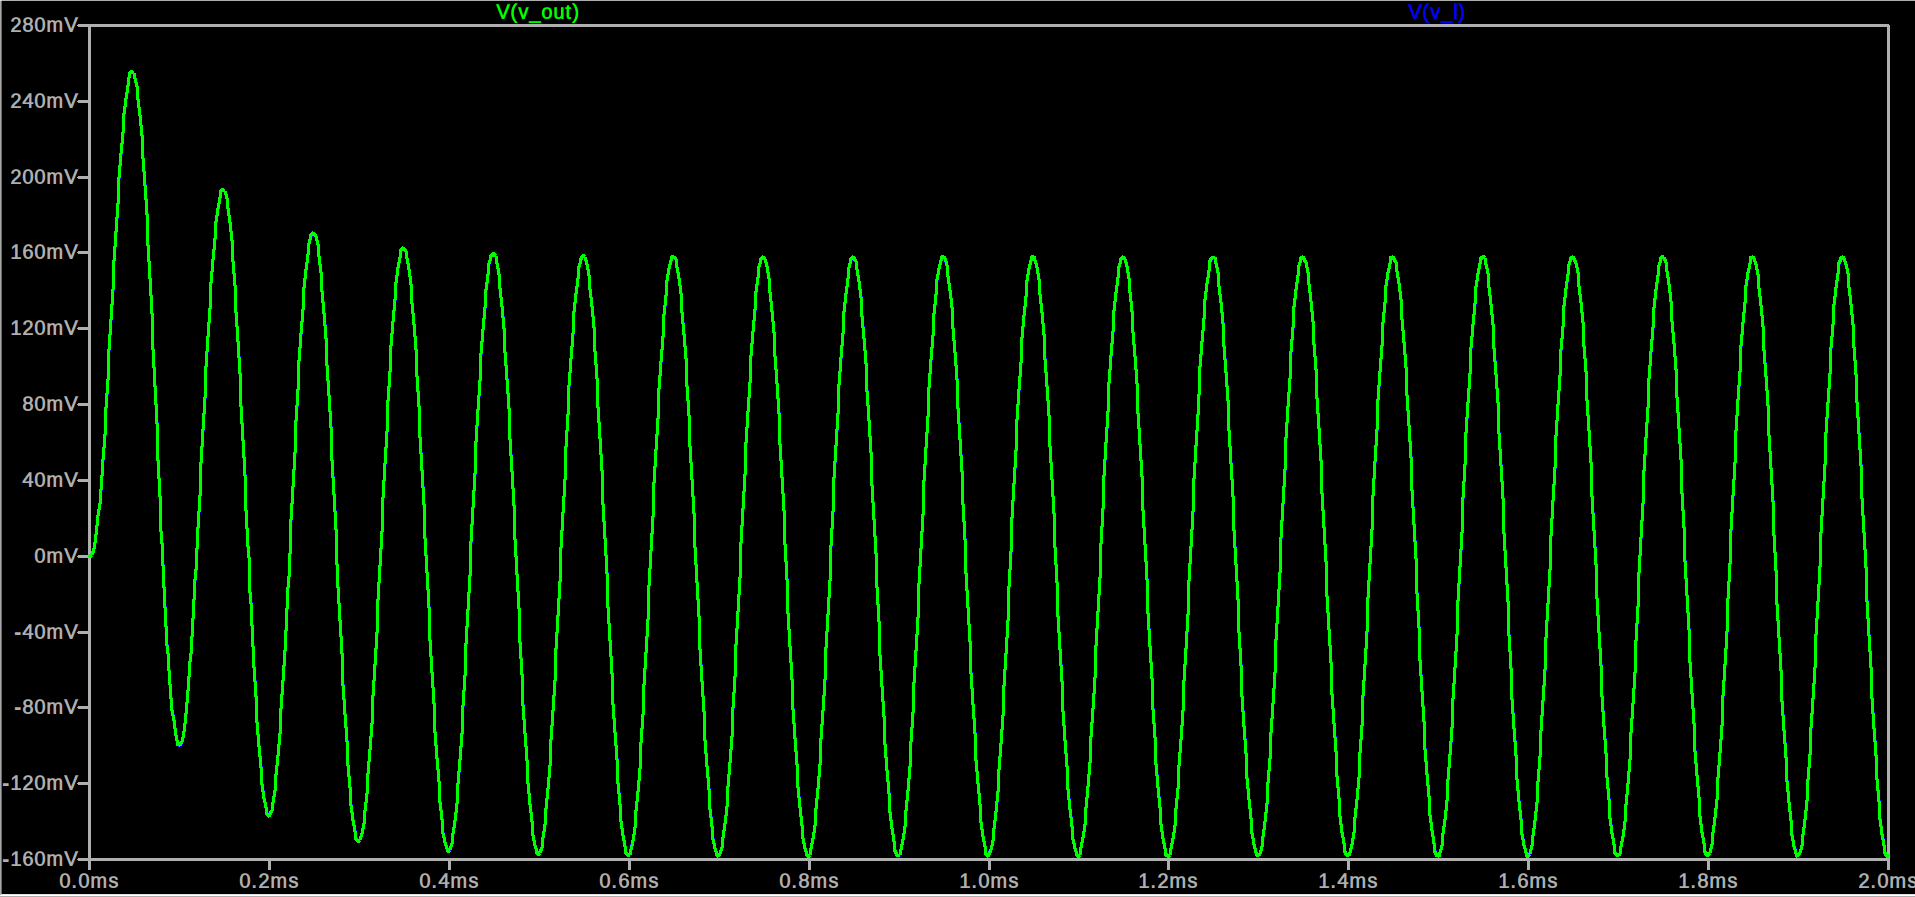
\includegraphics[width=1\textwidth]{assets/rlc-sin-transient-out.png}
    \caption{$V_{out}$ Transient Response}
    \label{fig:rlc_v_out_transient}
\end{figure}

\begin{figure}[h]
    \centering
    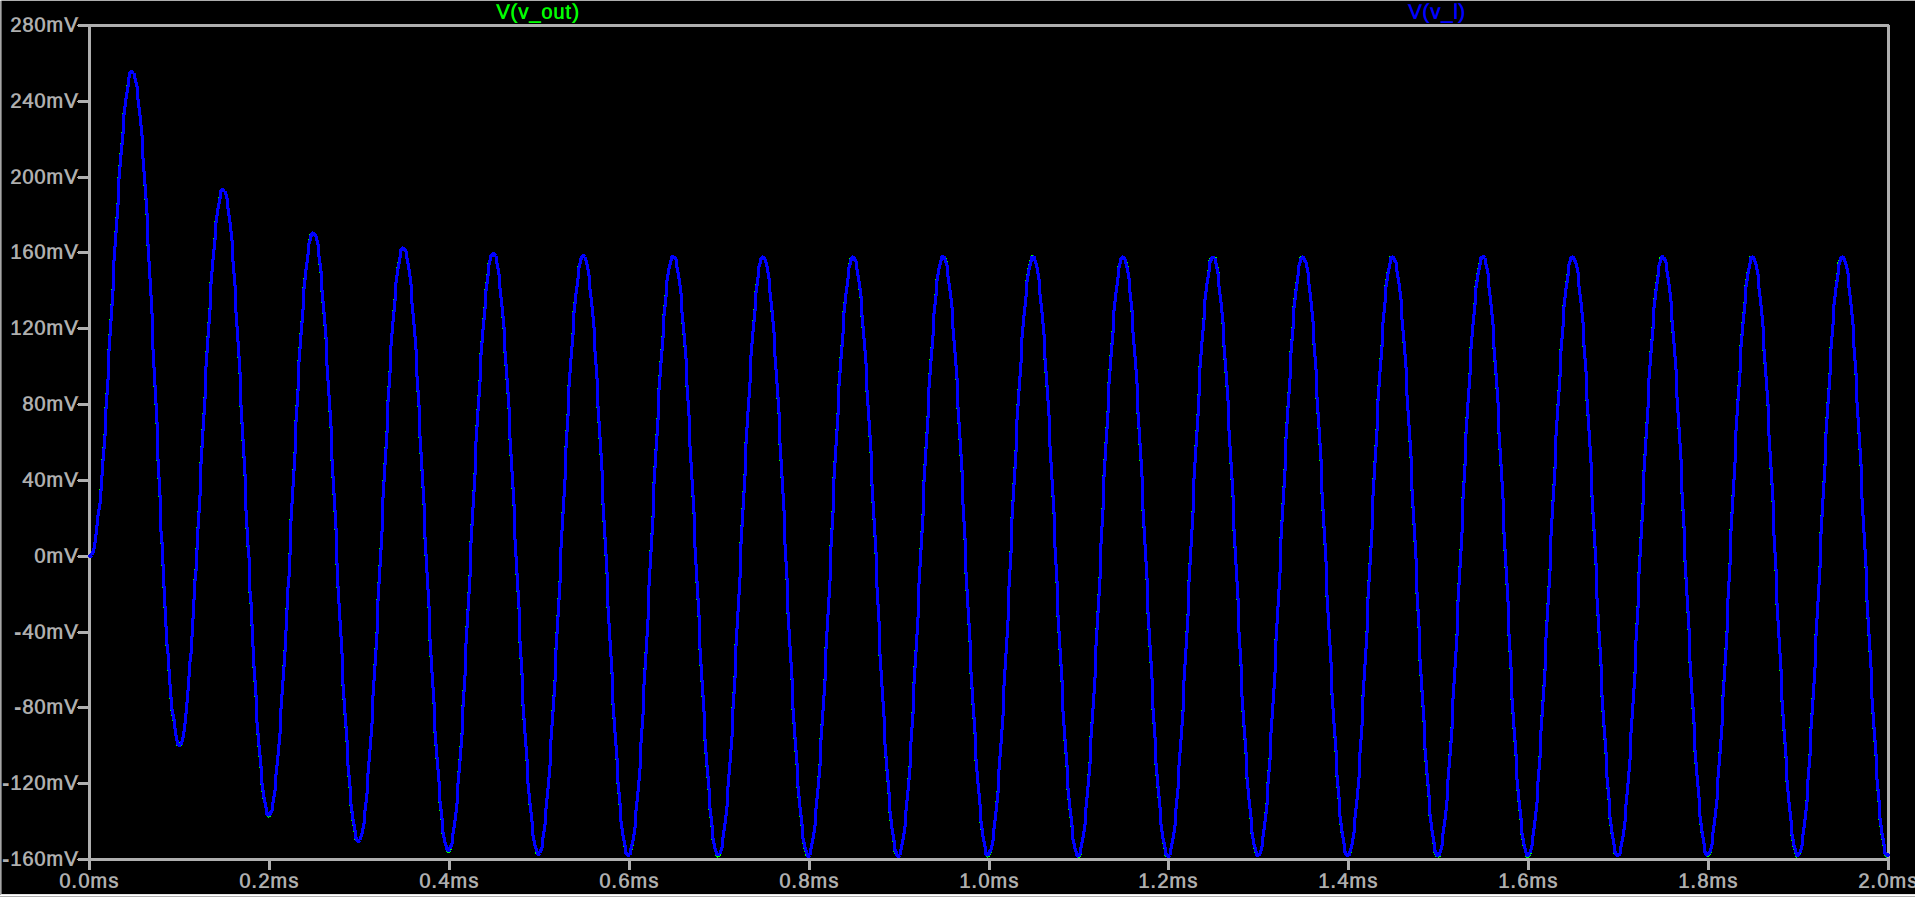
\includegraphics[width=1\textwidth]{assets/rlc-sin-transient-laplace.png}
    \caption{$H_{V}(s)$ Transient Response}
    \label{fig:rlc_v_laplace_transient}
\end{figure}

As shown in Figure \ref{fig:rlc_v_out_transient}, output voltage matches the transfer function $H_{V}(s)$ as shown in Figure \ref{fig:rlc_v_laplace_transient}.

\newpage
\thispagestyle{plain}

\subsection{Unit Step Response}
Unit step response can show the transient behavior of the circuit. In order to find unit step response, Heaviside step function ($u(t)$) is used as input voltage.

\begin{figure}[h]
    \centering
    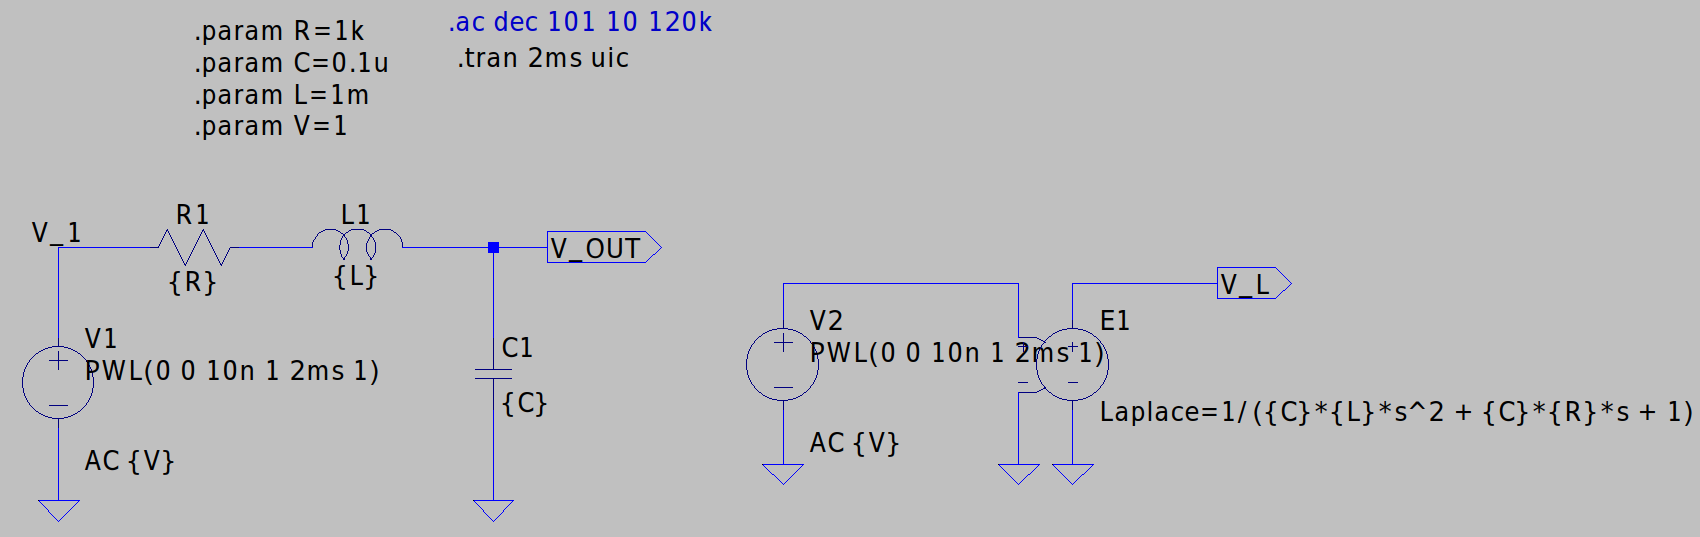
\includegraphics[width=1\textwidth, height=0.4\textheight]{assets/rlc-unit-step-sim.png}
    \caption{Unit Step Response Simulation Setup}
    \label{fig:unit_step_response}
\end{figure}

\newpage
\thispagestyle{plain}

\begin{figure}[h]
    \centering
    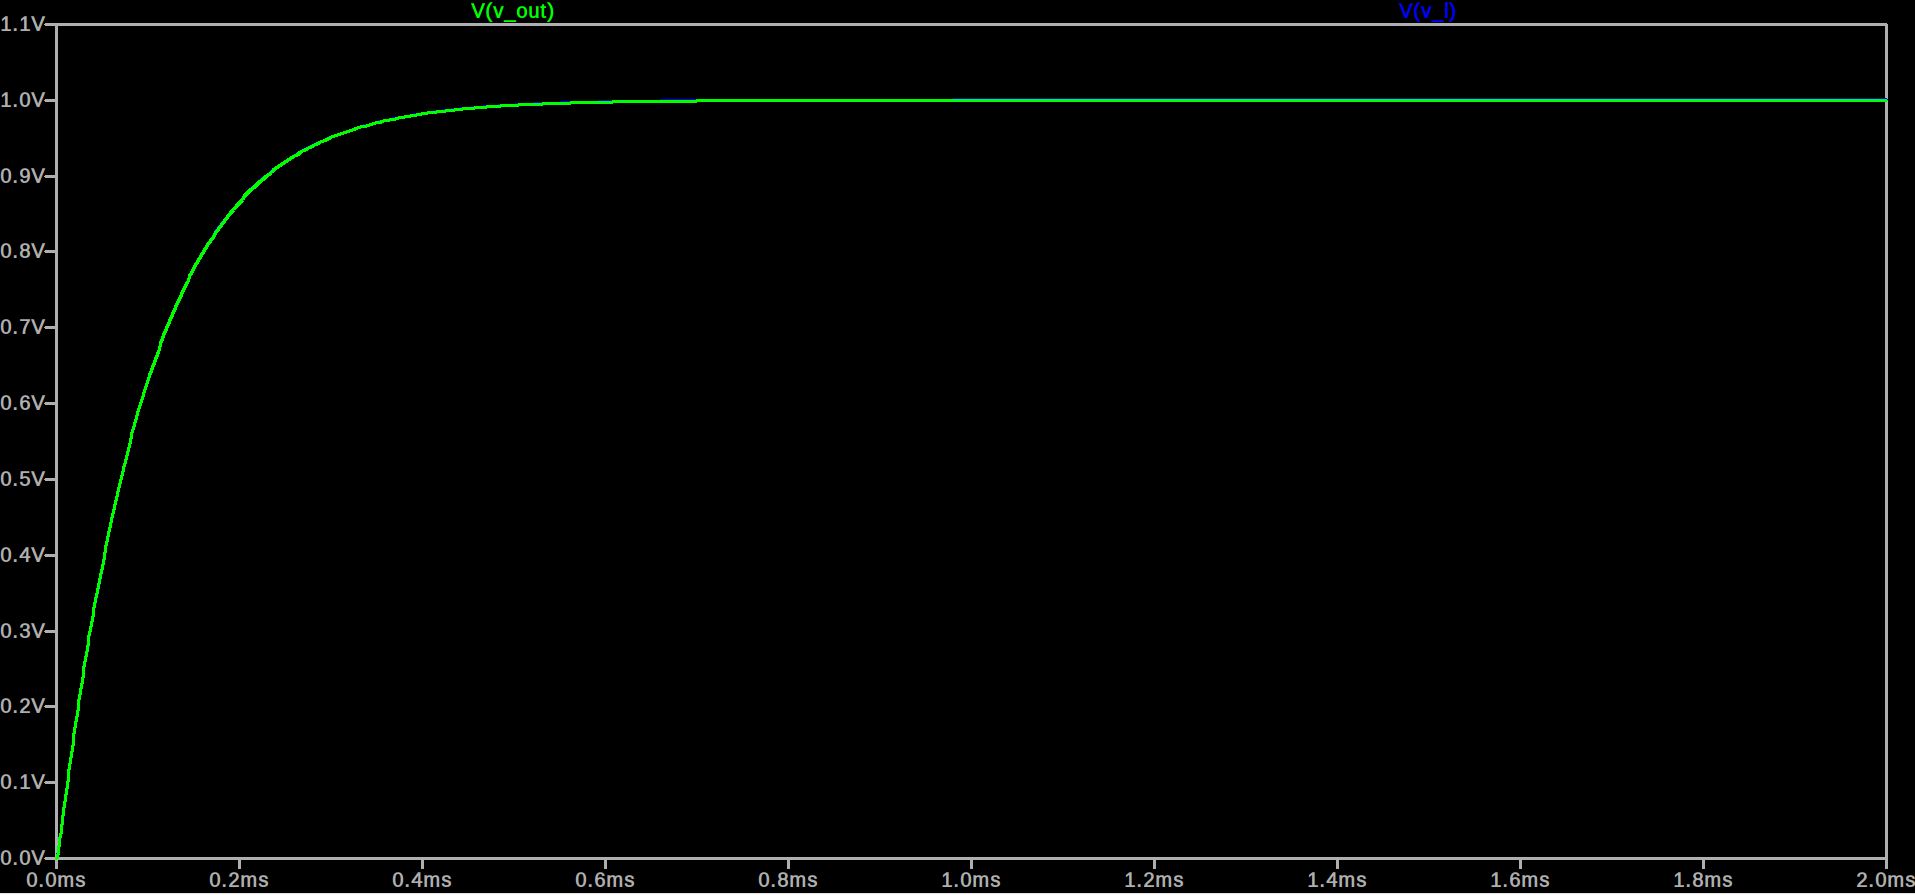
\includegraphics[width=1\textwidth]{assets/rlc-unit-step-sim-v-out.png}
    \caption{$V_{out}$ Unit Step Response}
    \label{fig:rlc_v_out_unit_step_response}
\end{figure}

\begin{figure}[h]
    \centering
    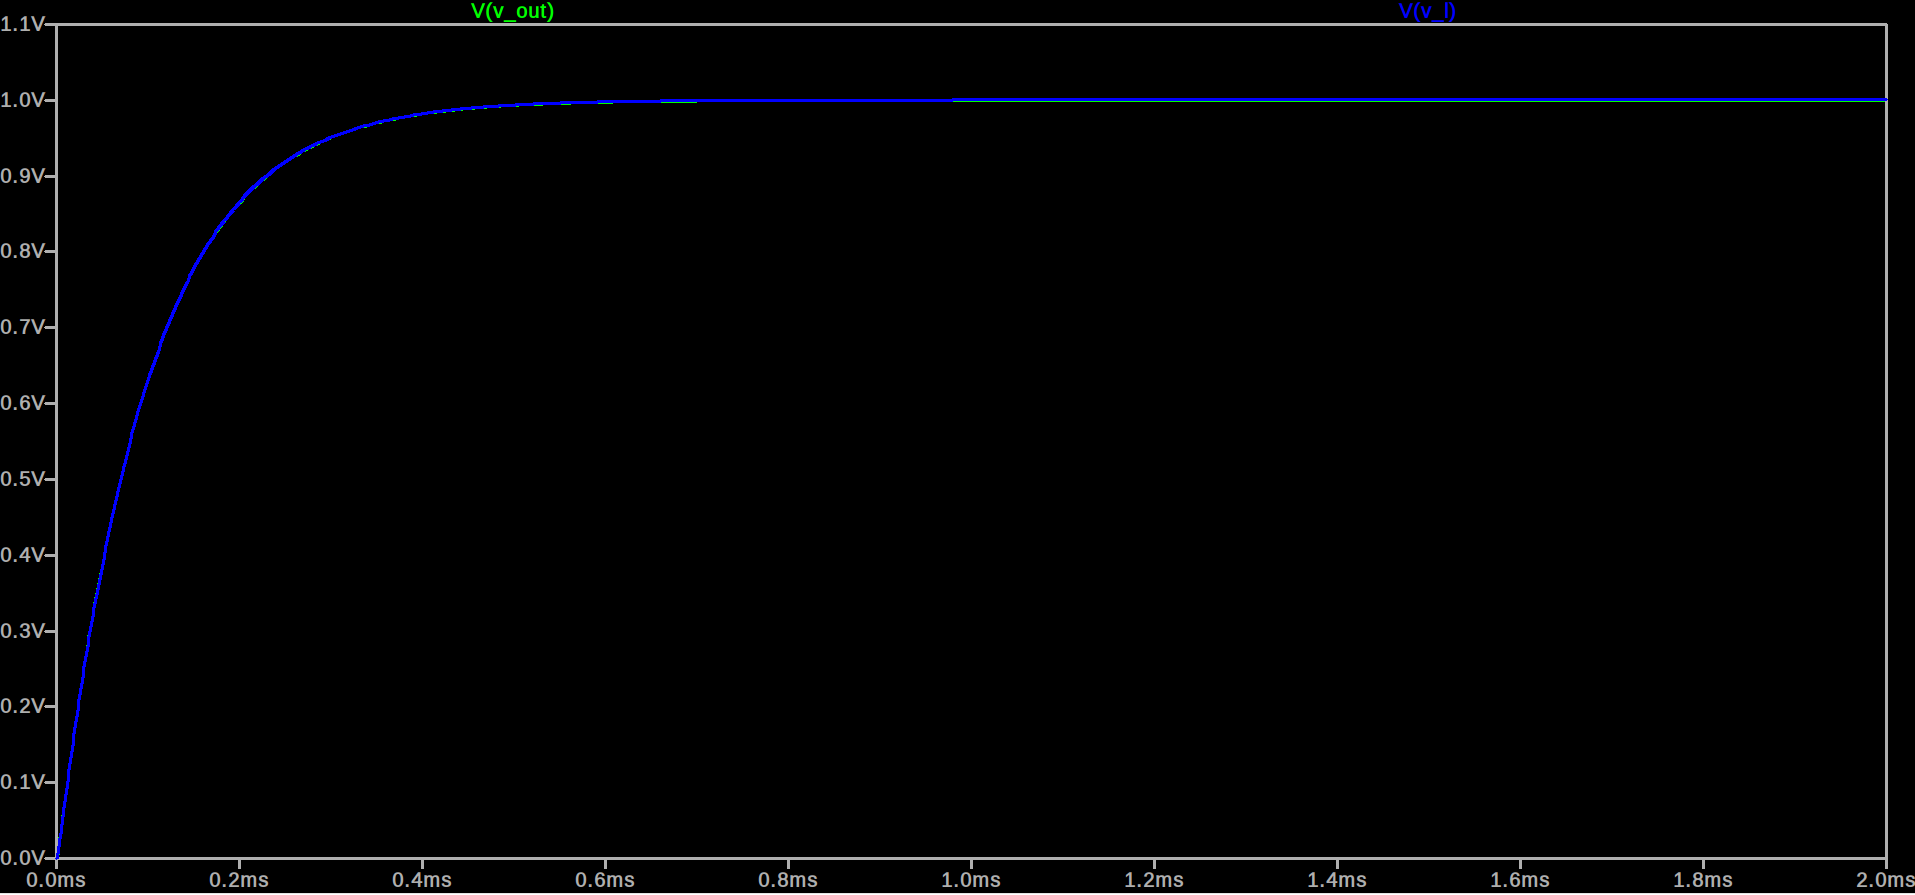
\includegraphics[width=1\textwidth]{assets/rlc-unit-step-sim-v-laplace.png}
    \caption{$H_{V}(s)$ Transient Response}
    \label{fig:rlc_v_laplace_unit_step_response}
\end{figure}

As shown in Figure \ref{fig:rlc_v_out_unit_step_response}, output voltage matches the transfer function $H_{V}(s)$ as shown in Figure \ref{fig:rlc_v_laplace_unit_step_response}.

\newpage
\thispagestyle{plain}

\section{Op-Amp Circuit Analysis}

\subsection{Transfer Function Derivation}
In order to derive the voltage gain transfer function ($H_{V}(s)$), we must first convert the circuit from time domain to the s-domain. The circuit is shown in Figure \ref{fig:op_amp_circuit}.

\begin{figure}[h]
    \centering
    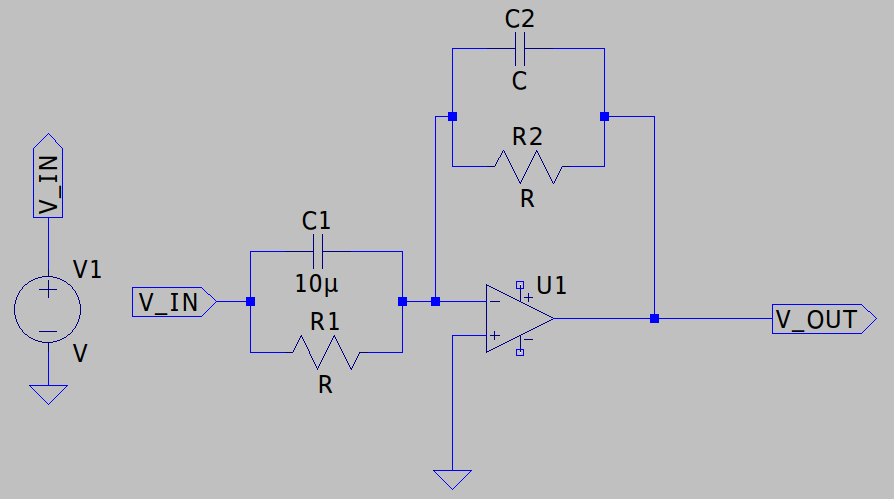
\includegraphics[width=1\textwidth]{assets/opamp-circ.png}
    \caption{Op-Amp Circuit}
    \label{fig:op_amp_circuit}
\end{figure}

\noindent Expected transfer function is $H_{V}(s) = \frac{V_{o}}{V_{i}} = -\frac{s+1000}{2(s+4000)}$:


\begin{align*}
    \text{let } Z_1 &= \frac{R_1}{1 + C_1 R_1 s} \\
    \text{let } Z_2 &= \frac{R_2}{1 + C_2 R_2 s} \\
    \frac{V_{in}}{Z_1} &= -\frac{V_{out}}{Z_2}\\
    V_{out} &= -\frac{Z_2}{Z_1} V_{in} \\
    \implies H_{V}(s) &= -\frac{Z_2}{Z_1} = -\frac{s+1000}{2(s+4000)} \\
    \frac{s+1000}{2(s+4000)} &= \frac{C_1}{C_2}\cdot \left[ \frac{s + \frac{1}{R_1 C_1}}{s + \frac{1}{R_2 C_2}} \right] \\
    \implies C_1 &= 10\mu F, C_2 = 20\mu F, R_1 = 100\Omega, R_2 = 12.5\Omega
\end{align*}

\newpage
\thispagestyle{plain}

Using these values, bode plot of the circuit and transfer function is shown below:

\begin{figure}[h]
    \centering
    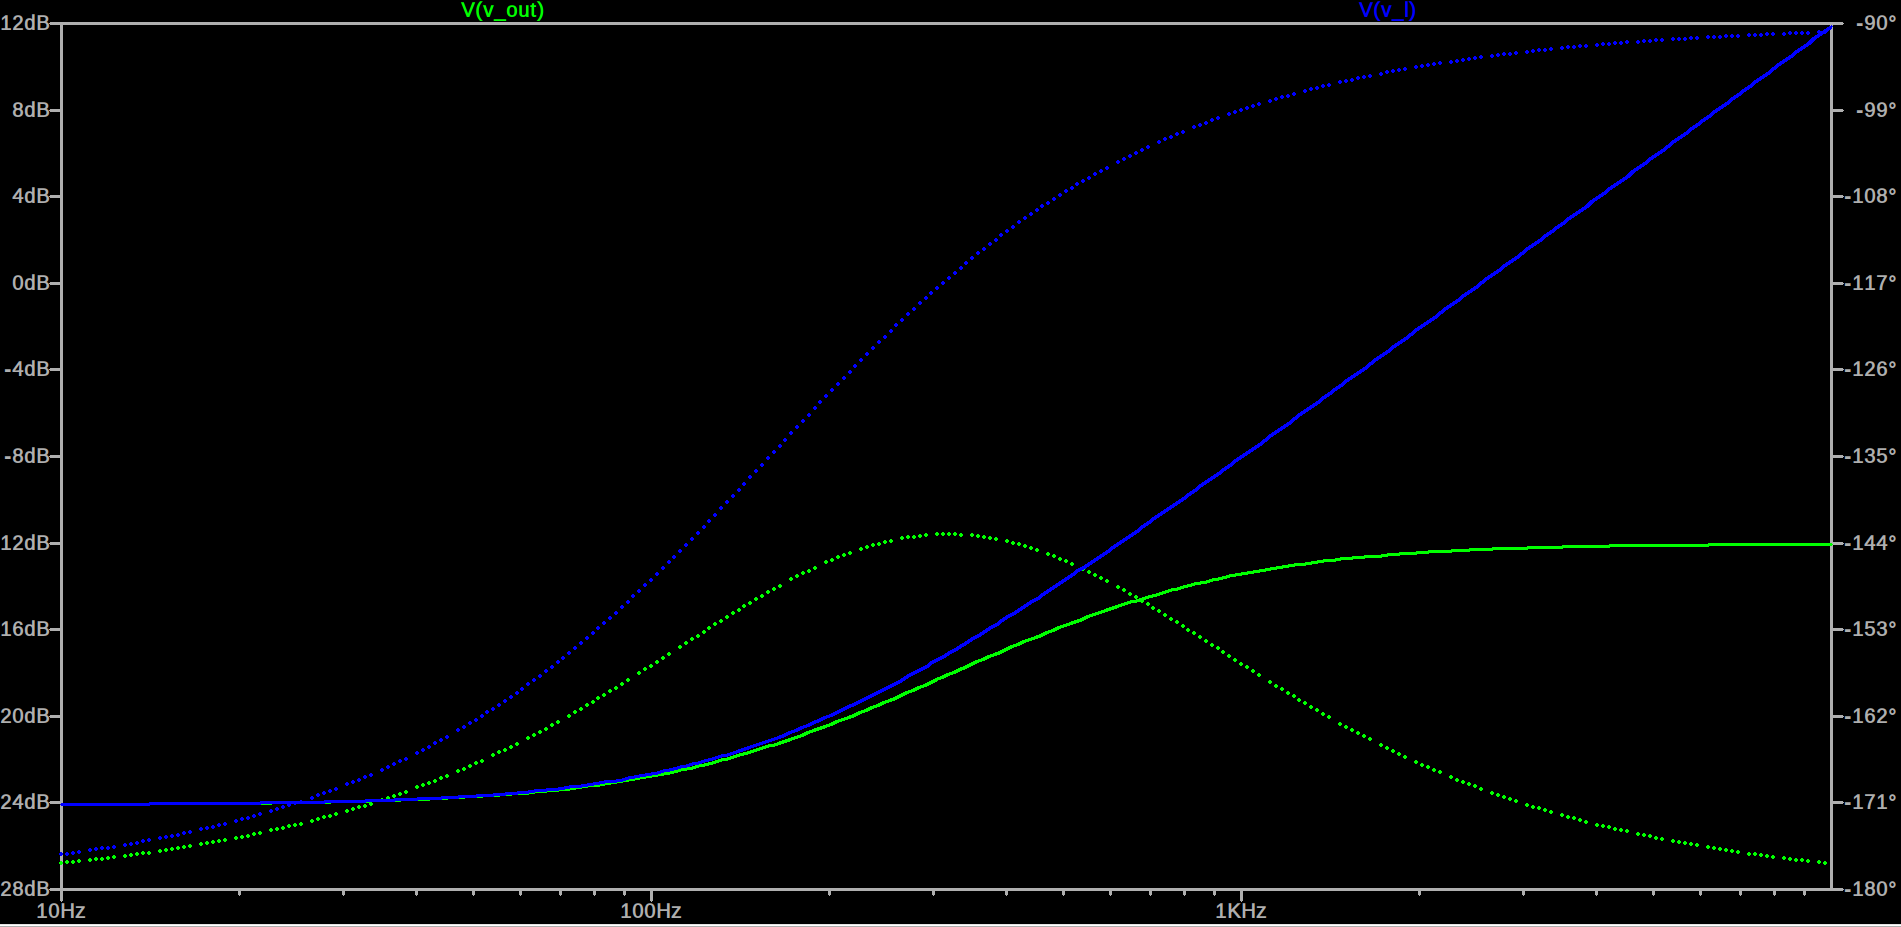
\includegraphics[width=1\textwidth]{assets/opamp-out-q.png}
    \caption{$V_{out}$ \& $H(s)$ Bode Plot}
    \label{fig:op_amp_v_out_bode_plot}
\end{figure}

As can be seen in Figure \ref{fig:op_amp_v_out_bode_plot}, output bode plot does not match the transfer function. This is due to pole and zero locations.

\begin{itemize}
    \item \textbf{Pole at $s=-4000$:}
        \begin{itemize}
            \item Pole has negative real part, meaning system is stable. The output will decay over time rather than growing unbounded.
            \item The pole at $s=-4000$ ensures the output responds quickly to changes.
        \end{itemize}
    \item \textbf{Zero at $s=-1000$:} 
        \begin{itemize}
            \item Zero has negative real part, meaning it adds a notch or dip in the frequency response.
            \item The zero at $s=-1000$ might suppress or attenuate frequencies associated with noise or other disturbances.
        \end{itemize}
    \item \textbf{Stability:} The system is stable as all poles have negative real part.
\end{itemize}

\newpage
\thispagestyle{plain}

\begin{figure}[h]
    \centering
    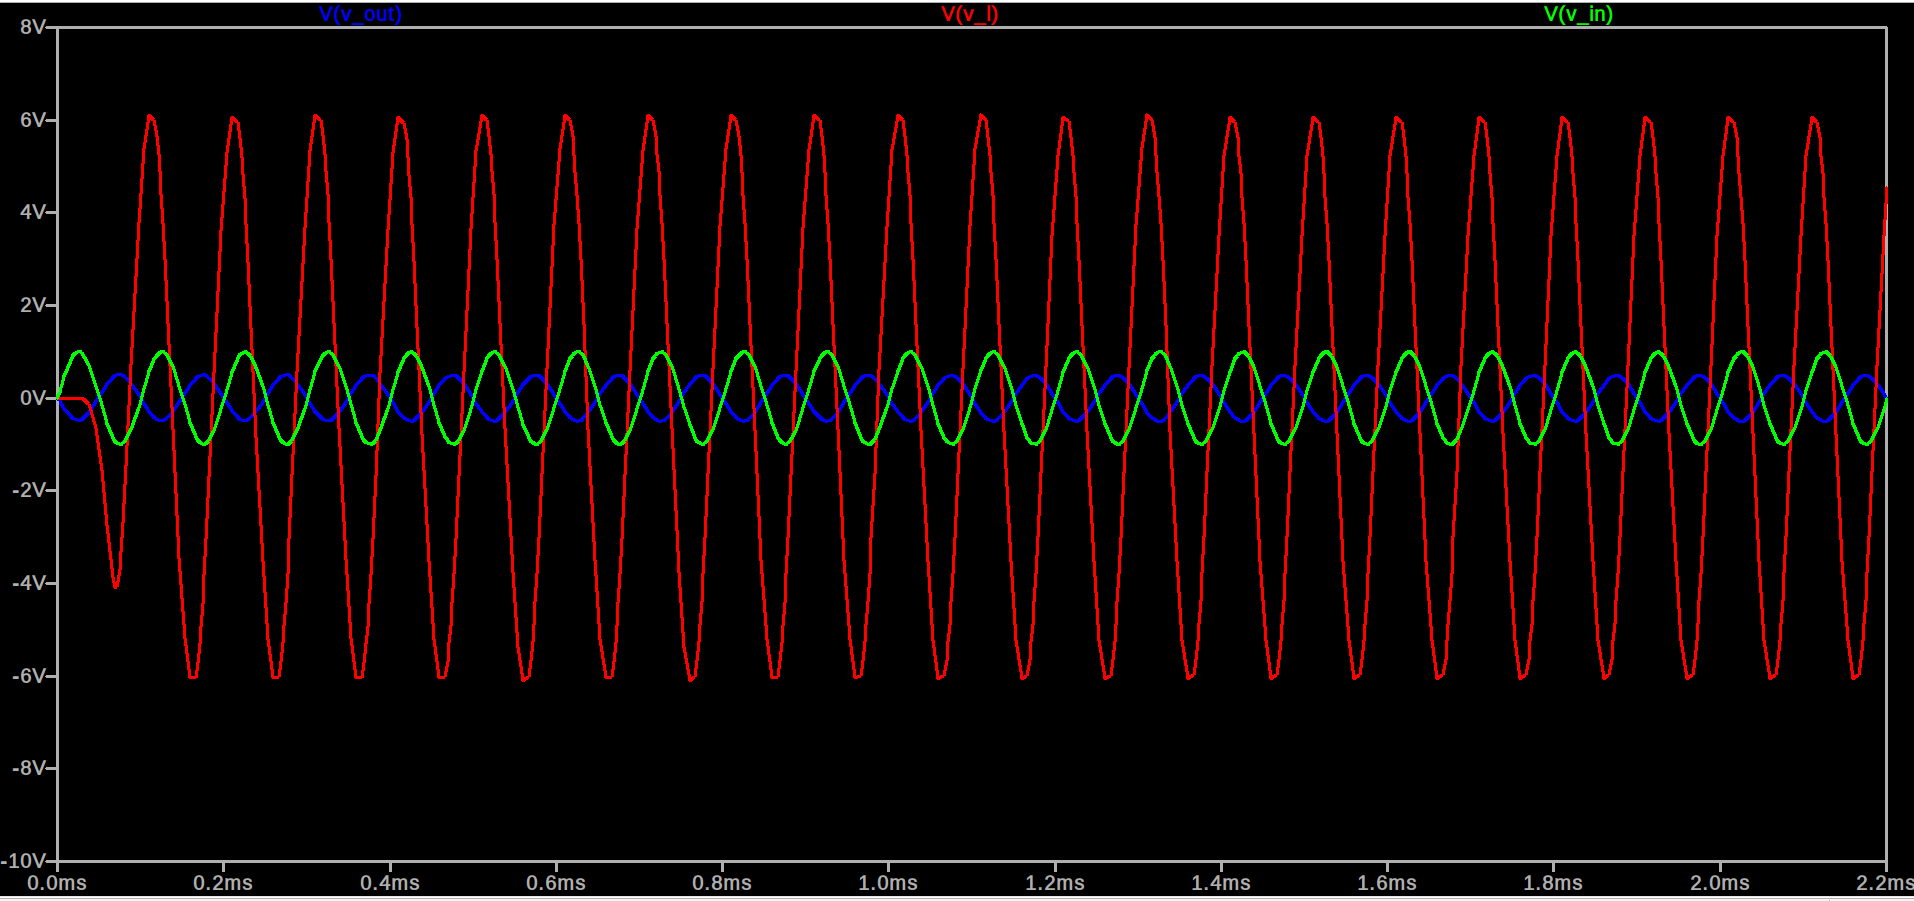
\includegraphics[width=1\textwidth]{assets/opamp-10k.png}
    \caption{$V_{in}$, $V_{out}$ \& $H(s)$ Plot @ $10kHz$}
    \label{fig:op_amp_out_10k}
\end{figure}

\begin{figure}[h]
    \centering
    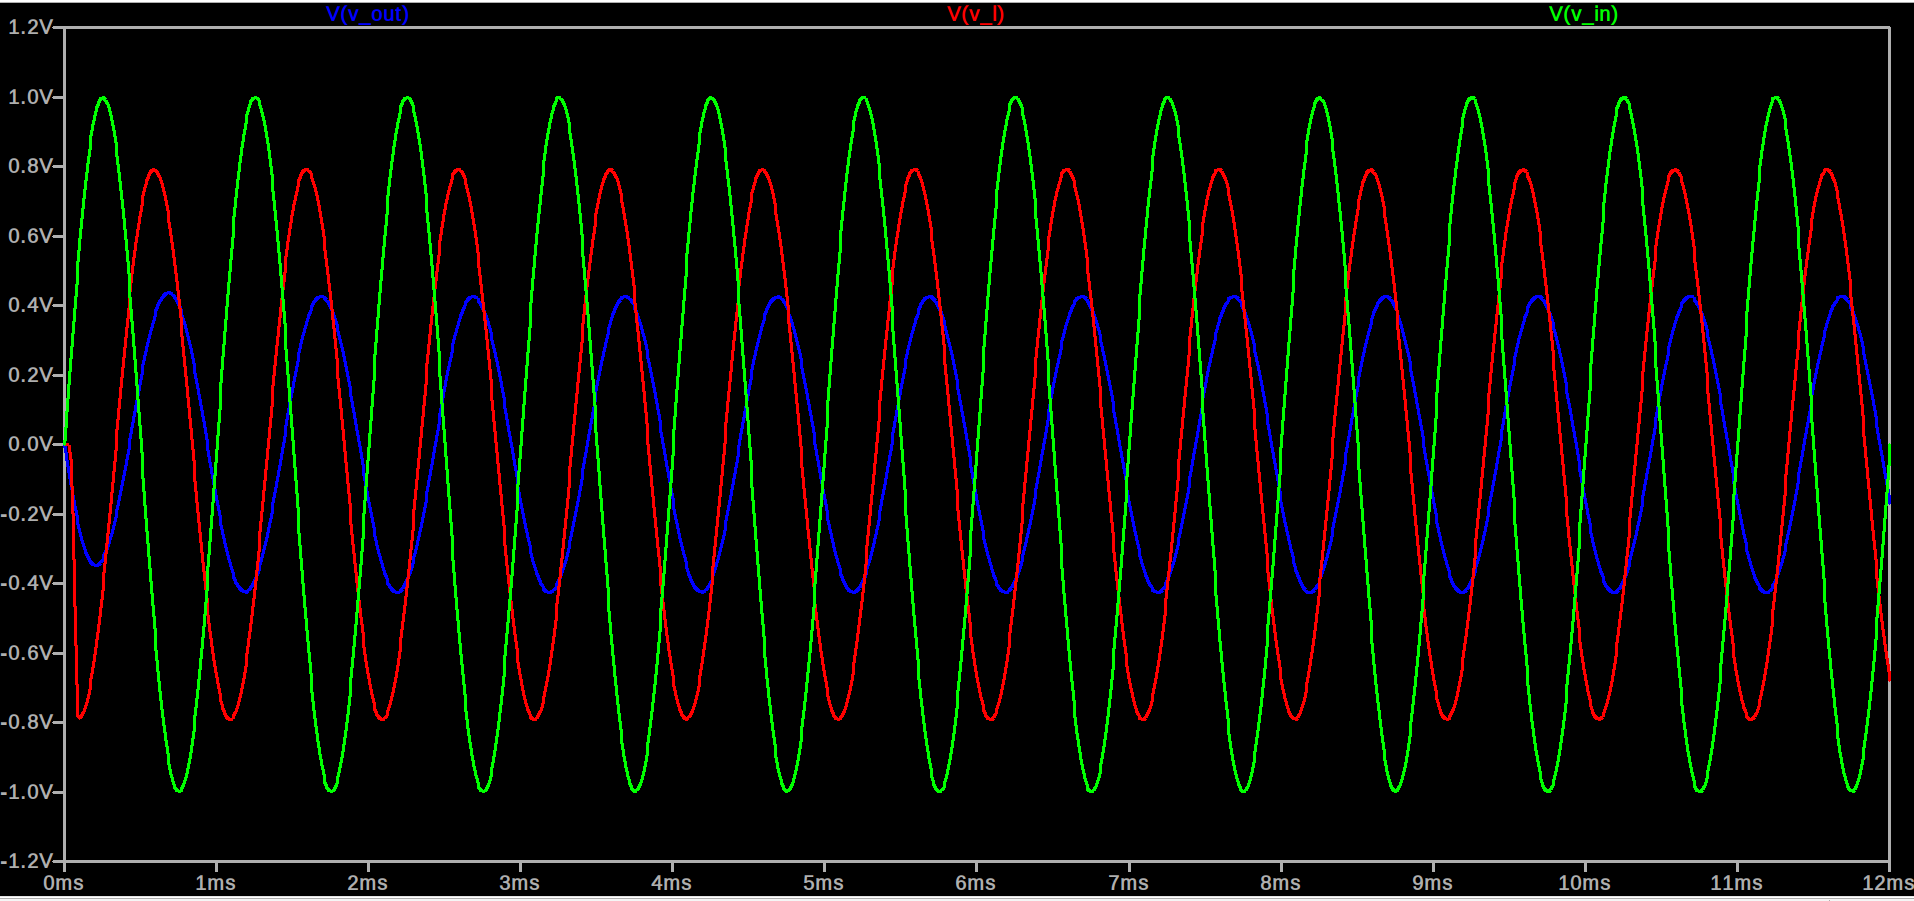
\includegraphics[width=1\textwidth]{assets/opamp-1k.png}
    \caption{$V_{in}$, $V_{out}$ \& $H(s)$ Plot @ $1kHz$}
    \label{fig:op_amp_out_1k}
\end{figure}

\newpage
\thispagestyle{plain}

\begin{figure}[h]
    \centering
    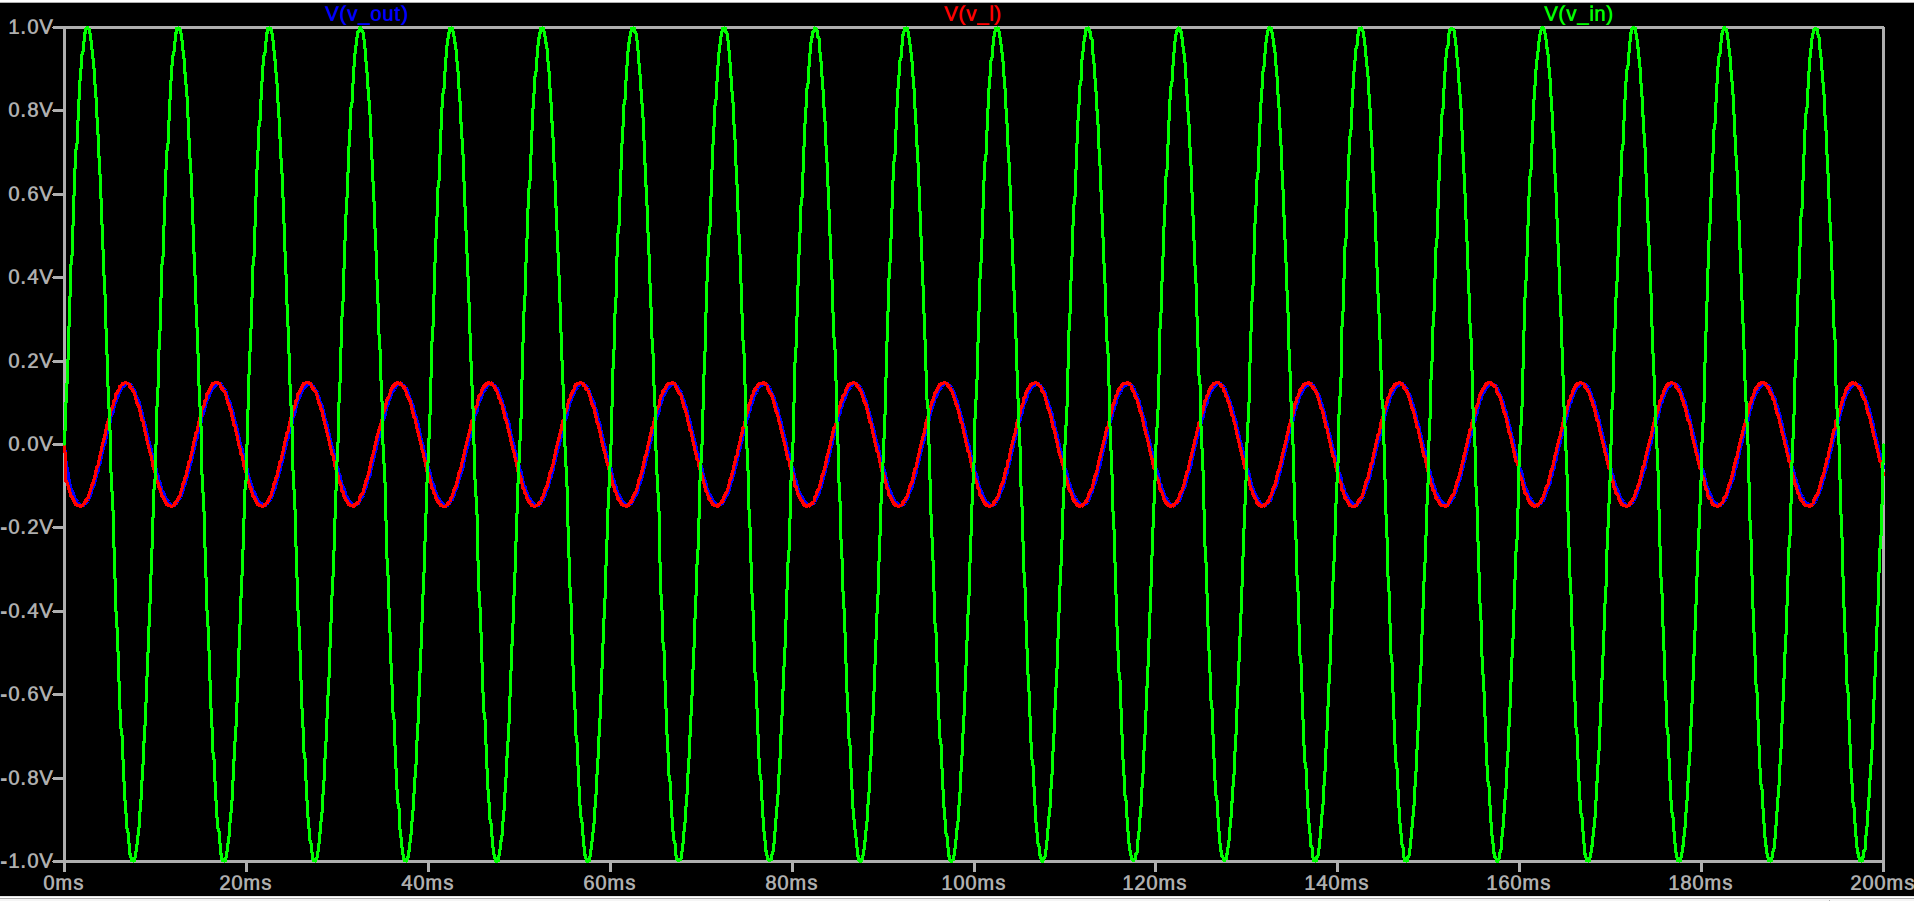
\includegraphics[width=1\textwidth]{assets/opamp-100.png}
    \caption{$V_{in}$, $V_{out}$ \& $H(s)$ Plot @ $100Hz$}
    \label{fig:op_amp_out_100}
\end{figure}

Plots seen in Figures \ref{fig:op_amp_out_10k}, \ref{fig:op_amp_out_1k}, and \ref{fig:op_amp_out_100} show the input and output voltages at $10kHz$, $1kHz$, and $100Hz$ respectively. These graphs confirms the bode plot in Figure \ref{fig:op_amp_v_out_bode_plot}.
